% :vim:set sw=2:
\newcommand{\linksize}{\scriptsize}
%\newcommand{\textrightarrow}{$\,\to\,$}
\begin{document}

\begin{frame}[plain]
  \titlepage
\end{frame}

\begin{frame}
  \frametitle{Who am I?}
  \begin{itemize}
    \item \href{mailto:alvherre@kurilemu.de}{Álvaro Herrera \texttt{<alvherre@kurilemu.de>}}
    \item Postgres contributor since 2002
    \item Working as a Postgres developer for 2ndQuadrant/EDB since 2012
    \item Worked on a number of SLRU-related projects:
      \begin{itemize}
	\item savepoints
	\item multixacts
	\item commit timestamps
      \end{itemize}
    \item \linksize I also came up with autovacuum, background workers, BRIN indexes, and more
    \begin{itemize} \item \linksize Feel free to grab hold of me on hallways to talk about stuff \end{itemize}
  \end{itemize}
\end{frame}

\begin{frame}
  \frametitle{Talk structure}
  \begin{enumerate}
    \item Historical review of SLRU development
    \item Report of an SLRU performance problem
    \item Development of the solution, step by step
    \item New Parameters in Postgres 17
    \item Call to Action and Future work
  \end{enumerate}
\end{frame}

\begin{frame}
   \frametitle{What {\bf is} an SLRU?}
   \begin{itemize}
     \item A very bad name for user-visible feature
      \item {\bf S}imple {\bf L}east {\bf R}ecently {\bf U}sed
      \item A mechanism to store transactional metadata
	 \begin{itemize}
	    \item And things with similar behavior
	 \end{itemize}
      \item Examples:
	 \begin{itemize}
	    \item Transaction commit/abort status
	    \item LISTEN / NOTIFY data
	    \item transaction commit times
	 \end{itemize}
      \item Keeps memory buffer of on-disk data
   \end{itemize}
\end{frame}

\section{Historical review of SLRU development}
\begin{frame}
  \sectionpage
\end{frame}


\begin{frame}
  \frametitle{Development History: 1. \texttt{pg\_clog}}
  % Mailing list thread: https://www.postgresql.org/message-id/flat/8382.973291660%40sss.pgh.pa.us
  \begin{itemize}
    \item Problem in Postgres 7.1: after 4 billion transactions, your database ist total kaputt \footnote{%
	\fontsize{6}{8}\selectfont \href{https://www.postgresql.org/message-id/flat/8382.973291660\%40sss.pgh.pa.us}
	{Transaction ID wraparound: problem and proposed solution (Fri 03 Nov 2000) \faExternalLink}}
      \item Why? 32-bit integer wraparound!

      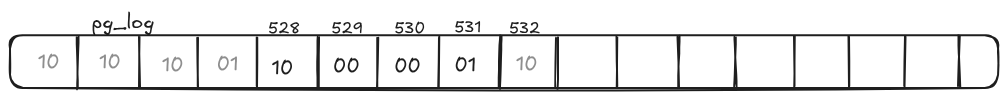
\includegraphics[width=0.85\textwidth]{pg_log.png}
  \end{itemize}
\end{frame}

\begin{frame}
  \frametitle{Transaction status storage}
  \begin{itemize}
    \item Reading a tuple requires looking up status of its creating
	    and deleting transactions
  
\includegraphics[width=0.7\textwidth]{tuple0.png}

\item Two bits per transaction id (xid):
  \begin{itemize}
    \item 00 \textrightarrow{} ``in-progress''
    \item 01 \textrightarrow{} ``aborted''
    \item 10 \textrightarrow{} ``committed''
  \end{itemize}
  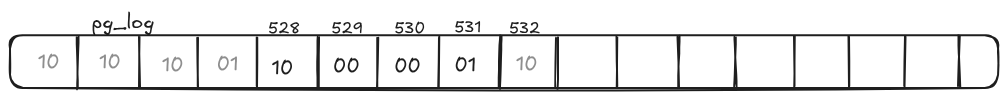
\includegraphics[width=0.85\textwidth]{pg_log.png}
  \end{itemize}

\end{frame}

\begin{frame}
  \frametitle{Development History: 1. \texttt{pg\_clog} (2)}

  \begin{itemize}
    \item Fix: Simplistic \texttt{pg\_log} pseudo-relation is replaced with \texttt{pg\_clog}
    \item {\linksize \href{https://git.postgresql.org/cgit/postgresql.git/commit/?id=2589735da08c4e597accb6eab5ae65b6339ee630}
      {Commit 2589735da08c: \faExternalLink \\
      Replace implementation of pg\_log as a relation accessed through the buffer manager with 'pg\_clog', a specialized access method modeled on pg\_xlog. \\
      Tom Lane \\
      Sat Aug 25 2001, Postgres 7.2}}
  \end{itemize}
\end{frame}

\begin{frame}
  \frametitle{How does \texttt{pg\_clog} work}
  \includegraphics[width=0.85\textwidth]{pg_clog.png}
  \begin{itemize}
    \item 4 transactions per byte
    \item 32k transactions per 8kB page
    \item 32 pages per file
  \end{itemize}
\end{frame}

\begin{frame}
  \frametitle{How does \texttt{pg\_clog} work (2)}
  \begin{itemize}
    \item If transaction committed long enough ago, ``hint bits'' are set
      in the ``infomask''
      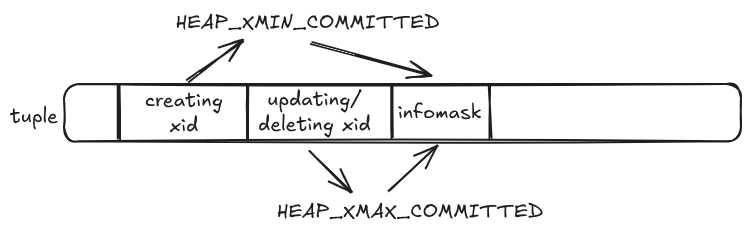
\includegraphics[width=0.80\textwidth]{tuple-hinted.png}
    \item When tuples are ``hinted'', no \texttt{pg\_clog} lookups are needed
    \item Old \texttt{pg\_clog} segments no longer needed
      \begin{itemize}
    \item ``wraparound'' is now possible!
      \end{itemize}
  \end{itemize}
\end{frame}

\begin{frame}
  \frametitle{How does \texttt{pg\_clog} work (3)}
  \begin{itemize}

    \item 8 in-memory pages store the status of $ 32768 * 8 = 262144 = 256k $ transactions
    \item At this point, LRU is an internal \texttt{pg\_clog} implementation detail
      \begin{itemize}
	\item \texttt{pg\_clog} no longer in \textit{shared buffers}, so a buffer management algorithm was needed
	\item LRU was open-coded in \texttt{clog.c}
      \end{itemize}
    \item[]
    \item Much later, \texttt{pg\_clog} was renamed \texttt{pg\_xact}, 
      commit \href{https://git.postgresql.org/cgit/postgresql.git/commit/?id=88e66d193fba}{88e66d193fba} (2017).
  \end{itemize}
\end{frame}


\begin{frame}
  \frametitle{Development History: 2. \texttt{slru.c}}
  \begin{itemize}
    \item My first big project: \texttt{SAVEPOINTS} (geb. ``nested transactions'')
    \item \texttt{slru.c} was born from \texttt{pg\_clog} to support this
    \item {\linksize \href{https://git.postgresql.org/cgit/postgresql.git/commit/?id=0abe7431c6d7a022e7f24a4f145c702900f56174}
      {Commit 0abe7431c6d7: \faExternalLink \\
      This patch extracts page buffer pooling and the simple least-recently-used strategy from clog.c into slru.c. \\
      Manfred Koizar (via Bruce Momjian) \\
      Wed Jun 11 2003, Postgres 7.4}}
    \item The term ``slru'' was invented at this point
    \item Nobody thought that this name would ever be exposed to users
\end{itemize}
\end{frame}

\begin{frame}
  \frametitle{Development History: 3. \texttt{pg\_subtrans}}
  \begin{itemize}
    \item Nested transactions
    \item {\linksize \href{https://git.postgresql.org/cgit/postgresql.git/commit/?id=573a71a5da70d6e2503c8f53e3b4f26b3b6d738d}
      {Commit 573a71a5da70: \faExternalLink \\
      Nested transactions. \\
      Álvaro Herrera, with some help from Tom Lane \\
      Thu Jul 1 2004, Postgres 8.0}}
    \item First user of \texttt{slru.c} outside of \texttt{clog.c}
  \end{itemize}
\end{frame}

\begin{frame}
  \frametitle{Is transaction XYZ running? (no subtransactions)}
  Without subtransactions, knowing whether a transaction is running
  is easy, it only requires reading memory:
  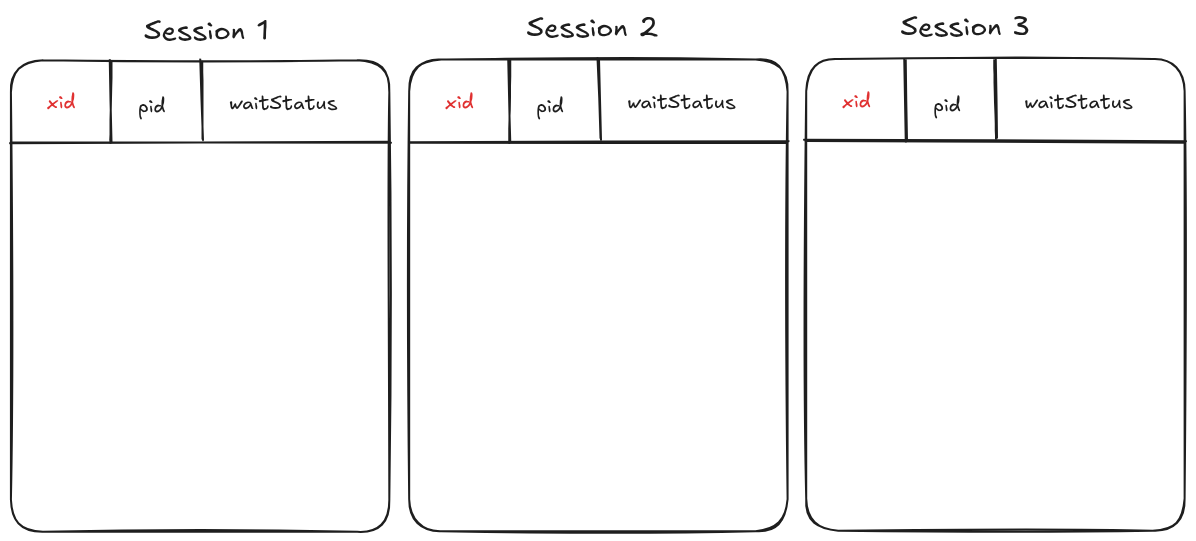
\includegraphics[width=0.8\textwidth]{pgproc-no-subxids.png}
\end{frame}

\begin{frame}
  \frametitle{Is transaction XYZ running? (w/ subtransactions)}
  \center 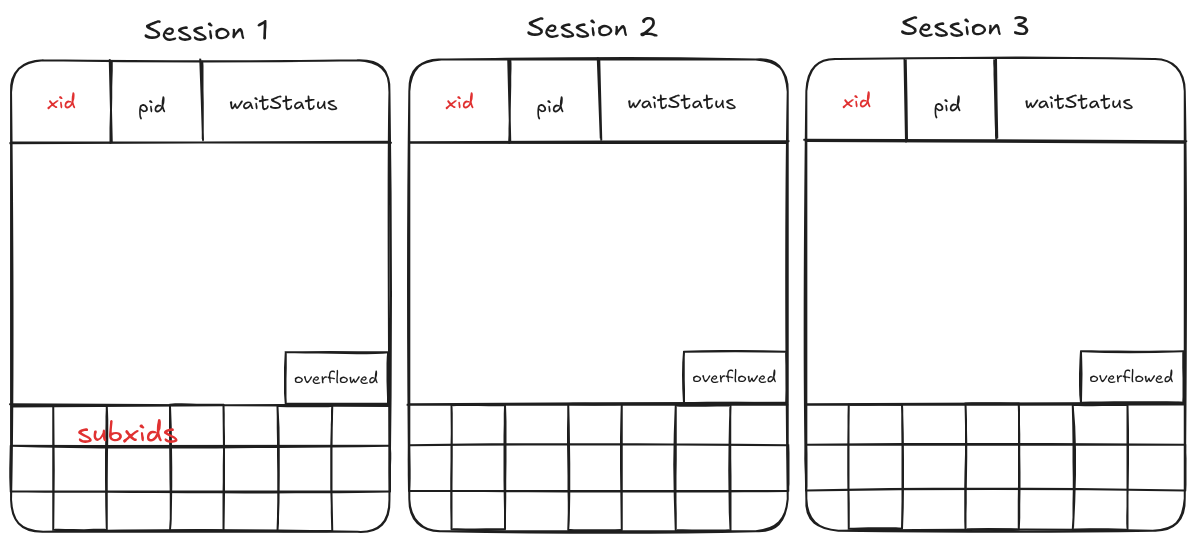
\includegraphics[width=0.7\textwidth]{pgproc-with-subxids.png}
  \begin{itemize}
    \item \texttt{pg\_subtrans} responds to ``is transaction X running?'' in presence of subtransactions
      \begin{itemize}
	\item ... only needed for transactions with >64 subtransactions
      \end{itemize}
  \end{itemize}
\end{frame}

\begin{frame}
  \frametitle{So what is \texttt{pg\_subtrans} \emph{for}?}
  \begin{itemize}
    \item \texttt{pg\_subtrans}: needed to store parent TransactionId for each \textit{subtransaction}
    \item 4 bytes per transaction (16x larger than \texttt{pg\_clog}!)
    \item 8 pages of 8kB each have room for 16k transactions
  \end{itemize}
  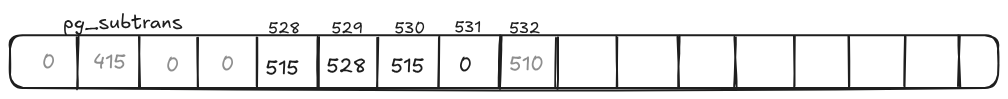
\includegraphics[width=0.85\textwidth]{pg_subtrans.png}
\end{frame}

\begin{frame}
  \frametitle{Development History: \texttt{pg\_multixact}}
   \begin{itemize}
      \item {\linksize \href{https://git.postgresql.org/cgit/postgresql.git/commit/?id=d1e027221d0243b7b57eabb0e482923dd7d1c8eb}
	{Commit d1e027221d02: \faExternalLink \\
	Implement sharable row-level locks, and use them for foreign key references to eliminate unnecessary deadlocks. \\
	Álvaro Herrera and Tom Lane \\
	Thu Apr 28 2005, Postgres 8.1}}
      \item {\texttt pg\_multixact}: A two-level mechanism to store
	variable-sized arrays using fixed-size \texttt{slru} addressing
   \end{itemize}
\end{frame}

\begin{frame}
  \frametitle{Foreign keys: avoiding SELECT FOR UPDATE}
  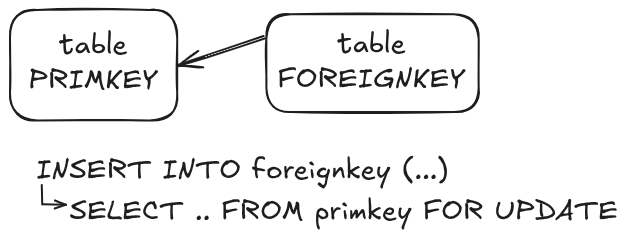
\includegraphics[width=0.8\textwidth]{select-for-update.png}
  \vspace{0.7cm}
  
\includegraphics[width=\textwidth]{tuple.png}
\end{frame}

\begin{frame}
  \frametitle{Foreign keys: SELECT FOR SHARE to the rescue}
  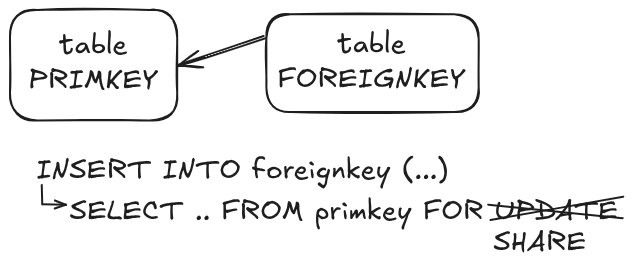
\includegraphics[width=0.8\textwidth]{select-for-share.png}
\end{frame}

\begin{frame}
  \frametitle{How does \texttt{pg\_multixact} work?}
  \begin{itemize}
    \item Each MultiXactId is a pointer to \texttt{pg\_multixact/offset}
    \item Each multixact offset is a pointer to \texttt{pg\_multixact/members}
    \item We know how many members to read by reading the offset after ours
  \end{itemize}

  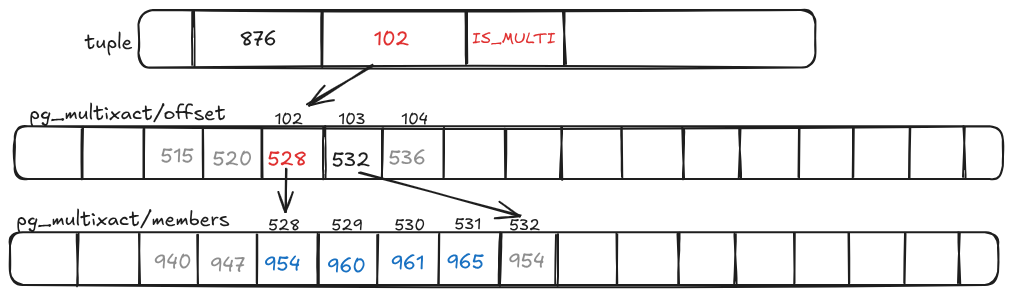
\includegraphics[width=\textwidth]{multixact.png}
\end{frame}

\begin{frame}
  \frametitle{Development History 5: Variable sized SLRUs}
  \begin{itemize}
    \item {\linksize \href{https://git.postgresql.org/cgit/postgresql.git/commit/?id=887a7c61f630}
      {Commit 887a7c61f630: \faExternalLink \\
      Get rid of slru.c's hardwired insistence on a fixed number of slots per
      SLRU area.  \alert<3>{The number of slots is still a compile-time constant (someday
      we might want to change that)}, but at least it's a different constant for
      each SLRU area.  \alert<2>{Increase number of subtrans buffers to 32 based on
      experimentation with a heavily subtrans-bashing test case, and increase
      number of multixact member buffers to 16, since it's obviously silly for
      it not to be at least twice the number of multixact offset buffers.} \\
      Tom Lane \\
      Tue Dec 6 2005, Postgres 8.2}}
  \end{itemize}
\end{frame}

\begin{frame}
  \frametitle{(Short) theory of operation}
  Why a small number of buffers?  Here's how it works:
  \begin{enumerate}
    \item With the SLRU control lock held:
    \item \alert<2>{Linearly scan the array of buffers} to see if one contains the page we want
    \item If we find it, we're done  % TODO mark the underline
    \item If not, the scan has chosen a ``victim'' buffer to evict (least recently used)
      \begin{enumerate}
	\item Evict it, leaving buffer free
	\item Load our page onto our buffer
	\item Increment ``recently used'' counter
      \end{enumerate}
    \item Now the page in buffer can be processed 
  \end{enumerate}
\end{frame}

\begin{frame}
  \frametitle{Development History 6: \texttt{pg\_notify}}
  \begin{itemize}
    \item \linksize {\href{https://git.postgresql.org/cgit/postgresql.git/commit/?id=d1e027221d0243b7b57eabb0e482923dd7d1c8eb}
      {Commit d1e027221d02: \faExternalLink \\
      Replace the pg\_listener-based LISTEN/NOTIFY mechanism with an in-memory
      queue. \\
      Joachim Wieland (via Tom Lane) \\
      Tue Feb 16 2010, Postgres 9.0}}
    \item This allowed NOTIFY to carry user-specified payload
    \item SLRU buffer of 8 pages
      \begin{itemize}
	\item ... but pages only have to be retained until all backends read notification messages
	\item ... which happens as soon as they run any command at all
	\item \sout{Small chances of overflowing the buffer}
      \end{itemize}
  \end{itemize}
\end{frame}

\begin{frame}
  \frametitle{Development History 7: \texttt{pg\_serial}}
   \begin{itemize}
     \item \linksize {\href{https://git.postgresql.org/cgit/postgresql.git/commit/?id=dafaa3efb75ce1aae2e6dbefaf6f3a889dea0d21}
       {Commit dafaa3efb75c: \faExternalLink \\
       Implement genuine serializable isolation level. \\
       Kevin Grittner and Dan Ports \\
       Tue Feb 8 2011, Postgres 9.1}}
     \item First SERIALIZABLE implementation using \emph{serializable snapshot isolation} (best in class)
     \item SLRU buffer of 16 pages
       \begin{itemize}
	 \item ... but lookups only occur once per command in serializable transactions
	 \item Much lower frequency
	 \item Each item is 8 bytes long
       \end{itemize}
   \end{itemize}
\end{frame}

\begin{frame}
  \frametitle{Development History 8: Make \texttt{pg\_clog} size adaptive}
  \begin{itemize}
     \item \linksize {\href{https://git.postgresql.org/cgit/postgresql.git/commit/?id=33aaa139e630}
       {Commit 33aaa139e630: \faExternalLink \\
       Make the number of CLOG buffers adaptive, based on shared\_buffers. \\
       Robert Haas \\
       Fri Jan 6 2012, Postgres 9.2}}
     \item First case of runtime-determined SLRU size
     \begin{itemize}
       \item 32 buffers with shared\_buffers = 128~MB and up
     \end{itemize}
   \item But not directly configurable!
  \end{itemize}
\end{frame}

\begin{frame}
  \frametitle{Development History: 9. \texttt{pg\_commit\_ts}}
  \begin{itemize}
    \item Commit Timestamps
     \item \linksize {\href{https://git.postgresql.org/cgit/postgresql.git/commit/?id=73c986adde5d73a5e2555da9b5c8facedb146dcd}
       {Commit 73c986adde5d: \faExternalLink \\
       Keep track of transaction commit timestamps \\
       Álvaro Herrera \\
       Wed Dec 3 2014, Postgres 9.5}}
     \item 12 bytes per entry
     \item For use with BDR
       \begin{itemize}
	 \item open-source bi-directional replication implementation
	 \item uses timestamp for simplistic conflict resolution
       \end{itemize}
     \item Size is adaptive like \texttt{pg\_clog}, but grows more slowly and the upper limit is smaller (16 buffers)
     \item (Theory behind this: not needed for long)
  \end{itemize}
\end{frame}

\begin{frame}
   \frametitle{What SLRUs exist}

   \begin{itemize}
      \item pg\_commit (neé pg\_clog), adaptive 8-32 pages
      \item pg\_subtrans, 32 pages
      \item pg\_multixact/offset, 8 pages
      \item pg\_multixact/members, 16 pages
      \item pg\_notify, 8 pages
      \item pg\_serial, 8 pages
      \item pg\_commit\_ts, adaptive 8-16 pages
      \item Total memory use: 88 pages = between 704 kB and 960 kB
   \end{itemize}
\end{frame}

\section{Moving Forward}
\begin{frame}
  \sectionpage
\end{frame}

\begin{frame}
  \frametitle{Borodin: Performance Problem Reported}
   Andrey Borodin reports to pgsql-hackers:
	 \begin{quote}
	    \linksize I'm investigating some cases of reduced database
	    performance due to MultiXactOffsetLock contention (80\%
	    MultiXactOffsetLock, 20\% IO DataFileRead).  The problem manifested
	    itself during index repack and constraint validation. Both being
	    effectively full table scans.
	 \end{quote}
	 {\linksize \href{https://postgr.es/m/2BEC2B3F-9B61-4C1D-9FB5-5FAB0F05EF86@yandex-team.ru}
	 {pgsql-hackers: MultiXact\textbackslash{}SLRU buffers configuration} \faExternalLink \\ (Fri, 8 May 2020) }
\end{frame}

\begin{frame}[fragile]
  \frametitle{Borodin: Performance Problem Reported (2)}

  \linksize
  \begin{verbatim}
database=# SELECT pid, wait_event, wait_event_type, state, query
database-# FROM pg_stat_activity    \watch 1
  pid  |         wait_event         | wait_event_type | state  |                       query
-------+----------------------------+-----------------+--------+----------------------------------------------------
 41344 | ClientRead                 | Client          | idle   | insert into t1 select generate_series(1,1000000,1)
 41375 | MultiXactOffsetControlLock | LWLock          | active | select * from t1 where i = ANY ($1) for share
 41377 | MultiXactOffsetControlLock | LWLock          | active | select * from t1 where i = ANY ($1) for share
 41378 |                            |                 | active | select * from t1 where i = ANY ($1) for share
 41379 | MultiXactOffsetControlLock | LWLock          | active | select * from t1 where i = ANY ($1) for share
 41381 |                            |                 | active | select * from t1 where i = ANY ($1) for share
 41383 | MultiXactOffsetControlLock | LWLock          | active | select * from t1 where i = ANY ($1) for share
 41385 | MultiXactOffsetControlLock | LWLock          | active | select * from t1 where i = ANY ($1) for share
(8 rows)
\end{verbatim}  
\end{frame}

\begin{frame}
  \frametitle{Borodin: Performance Problem Reported (3)}

  Andrey Borodin:
  \begin{quote}
I've found out that:

1. When MultiXact working set does not fit into buffers - benchmark results grow very high. Yet, very big buffers slow down benchmark
    too. For this benchmark optimal SLRU size [is] 32 pages for offsets and 64 pages for members (defaults are 8 and 16 respectively).
  \end{quote}

\end{frame}

\begin{frame}[fragile]
  \frametitle{Darold: Patch Benchmarking Results}
  \href{https://postgr.es/m/6ba7eae2-8b0c-0690-11a5-e921e6586180@darold.net}{Gilles Darold:}
  \linksize
  \begin{quote}
    Some time ago I have encountered a contention on MultiXactOffsetControlLock
    with a performance benchmark. Here are the wait event monitoring result with
    a polling each 10 seconds and a 30 minutes run for the benchmark:
  \end{quote}
  \begin{verbatim}
 event_type |           event            |   sum
------------+----------------------------+----------
 Client     | ClientRead                 | 44722952
 LWLock     | MultiXactOffsetControlLock | 30343060
 LWLock     | multixact_offset           | 16735250
 LWLock     | MultiXactMemberControlLock |  1601470
 LWLock     | buffer_content             |   991344
\end{verbatim}
\end{frame}


\begin{frame}[fragile]
  \frametitle{Darold: Patch Benchmarking Results (2)}
  Gilles Darold:
  \linksize 
  \begin{quote}
    After reading this thread I changed the value of the buffer size to 32 and 64 and obtain the following results:
  \end{quote}
  \begin{verbatim}
 event_type |           event            |    sum  
------------+----------------------------+-----------
 Client     | ClientRead                 | 268297572
 LWLock     | MultiXactMemberControlLock |  65162906
 LWLock     | multixact_member           |  33397714
 LWLock     | buffer_content             |   4737065
\end{verbatim}
\end{frame}


\begin{frame}[fragile]
  \frametitle{Darold: Patch Benchmarking Results (3)}
   Gilles Darold:
   \linksize 
   \begin{quote}
     I have increased the buffers to 128 and 512 and obtain the best
     results for this benchmark:

     Increasing buffer sizes to (128, 512)
   \end{quote}

   \begin{verbatim}
 event_type |           event            |    sum  
------------+----------------------------+-----------
 Client     | ClientRead                 | 160463037
 LWLock     | MultiXactMemberControlLock |   5334188
 LWLock     | buffer_content             |   5228256
 LWLock     | buffer_mapping             |   2368505
 LWLock     | SubtransControlLock        |   2289977
\end{verbatim}
\end{frame}

\begin{frame}
  \frametitle{Increasing Buffer Sizes is not Enough}
  Andrey Borodin again:
  % 494C5E7F-E410-48FA-A93E-F7723D859561@yandex-team.ru
  \linksize {
  \begin{quote}
    I have one more idea inspired by CPU caches.
    Let's make SLRU n-associative, where n \~{} 8.
    We can divide buffers into "banks", number of banks must be power of 2.
    All banks are of equal size. We choose bank size to approximately satisfy
    user's configured buffer size.
    Each page can live only within one bank. We use same search and eviction
    algorithms as we used in SLRU, but we only need to search/evict
    over 8 elements.
  \end{quote}
  }
  \begin{itemize}
    \item {\linksize \href{https://postgr.es/m/494C5E7F-E410-48FA-A93E-F7723D859561@yandex-team.ru}
      {pgsql-hackers: MultiXact\textbackslash{}SLRU buffers configuration \faExternalLink\\ (Sun, 11 Apr 2021)}}

    \item Dividing the buffers in \emph{banks} allows much larger buffer sizes
    \item ... without affecting performance of buffer search
  \end{itemize}
\end{frame}

\begin{frame}
  \frametitle{SLRU banks}
  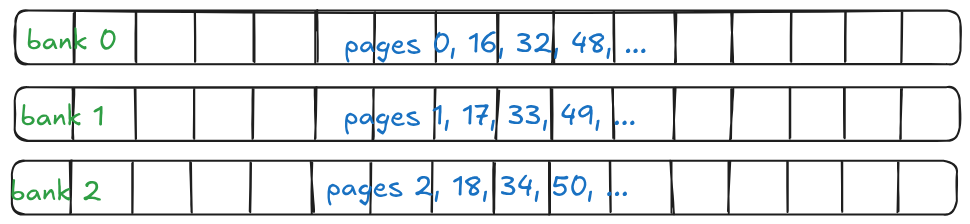
\includegraphics[width=0.9\textwidth]{banks.png}
\end{frame}

\begin{frame}
  \frametitle{Restricting the scan to banks}
  \begin{enumerate}
    \item \alert{With the bank lock held:}
    \item Linearly scan the array of buffers \alert{of the bank that contains the page} to see if one contains the page we want
    \item If we find it, \emph{we're done}
    \item If not, the scan has chosen a ``victim'' buffer to evict (least recently used)
      \begin{enumerate}
	\item Evict it, leaving buffer free
	\item Load our page onto our buffer
	\item Increment ``recently used'' counter
      \end{enumerate}
    \item Now the page in buffer can be processed 
  \end{enumerate}
\end{frame}

\begin{frame}
  \frametitle{New Kid in Town: \texttt{pg\_stat\_slru}}
  \begin{itemize}
    \item \texttt{pg\_stat\_slru} was born as the initial problem was being discussed
    \item {\linksize \href{https://git.postgresql.org/cgit/postgresql.git/commit/?id=28cac71bd368}
      {Commit 28cac71bd368: \faExternalLink \\
      Collect statistics about SLRU caches \\
      Tomas Vondra \\
      Thu Apr 2 2020, Postgres 13}}
    \item No motivation for this work was admitted other than healthy scientific curiosity
  \end{itemize}
\end{frame}

\begin{frame}[fragile]
  \frametitle{Example \texttt{pg\_stat\_slru}}

  \linksize
\begin{verbatim}
SELECT name, blks_zeroed, blks_hit, blks_read, blks_written
  FROM pg_stat_slru;

       name       │ blks_zeroed │  blks_hit   │ blks_read │ blks_written 
──────────────────┼─────────────┼─────────────┼───────────┼──────────────
 commit_timestamp │     1284048 │   387594150 │     54530 │      1305858
 multixact_member │       30252 │ 23852620477 │  48555852 │        26106
 multixact_offset │       10637 │ 23865848376 │  18434993 │         9375
 notify           │           0 │           0 │         0 │            0
 serializable     │           0 │           0 │         0 │            0
 subtransaction   │      513486 │ 12127027243 │ 153119082 │       431238
 transaction      │       32107 │ 22450403108 │  72043892 │        18064
 other            │           0 │           0 │         0 │            0
\end{verbatim}
  \linksize (``name'' column differs in versions prior to 17)

\end{frame}

\begin{frame}
  \frametitle{Finalizing a Solution}
  \begin{itemize}
    \item Dilip Kumar
      \href{https://postgr.es/m/CAFiTN-vzDvNz=ExGXz6gdyjtzGixKSqs0mKHMmaQ8sOSEFZ33A@mail.gmail.com}
      {further analyzed the problem \faExternalLink} as reported by customers, created
      additional pgbench reproducer workloads and posted a new proposal:
  \end{itemize}
  \begin{quote}
    \linksize Just increasing the size of the buffer pool doesn't necessarily help,
    because the linear search that we use for buffer replacement doesn't scale ...
  \end{quote}
  \begin{itemize}
    \item (We know!  Which is why the patch uses banks)
  \end{itemize}
  \begin{quote}
    \linksize
    ... and also because contention on the single centralized lock
    limits its scalability.
  \end{quote}
\end{frame}

\begin{frame}
  \frametitle{Proposed Changes to SLRUs}
  In addition to Andrey Borodin's ideas:
  \begin{itemize}
    \item Configurable buffer sizes
    \item Split each SLRU area in banks
  \end{itemize}

  Dilip Kumar proposed:
  \begin{itemize}
    \item Make the locking occur per bank rather than globally
    \item Modify operations to LRU counter to use atomic access
  \end{itemize}
\end{frame}

\begin{frame}
  \frametitle{Operating with atomics}
  \begin{enumerate}
    \item With the bank lock held:
    \item Linearly scan the array of buffers of the bank that contains the page to see if one contains the page we want
    \item If we find it, \emph{we're done}
    \item If not, the scan has chosen a ``victim'' buffer to evict (least recently used)
      \begin{enumerate}
	\item Evict it, leaving buffer free
	\item Load our page onto our buffer
	\item \alert{Increment ``recently used'' counter using atomic ops}
      \end{enumerate}
    \item Now the page in buffer can be processed 
  \end{enumerate}
\end{frame}

\begin{frame}
  \frametitle{Subtransaction TPS improvement}
  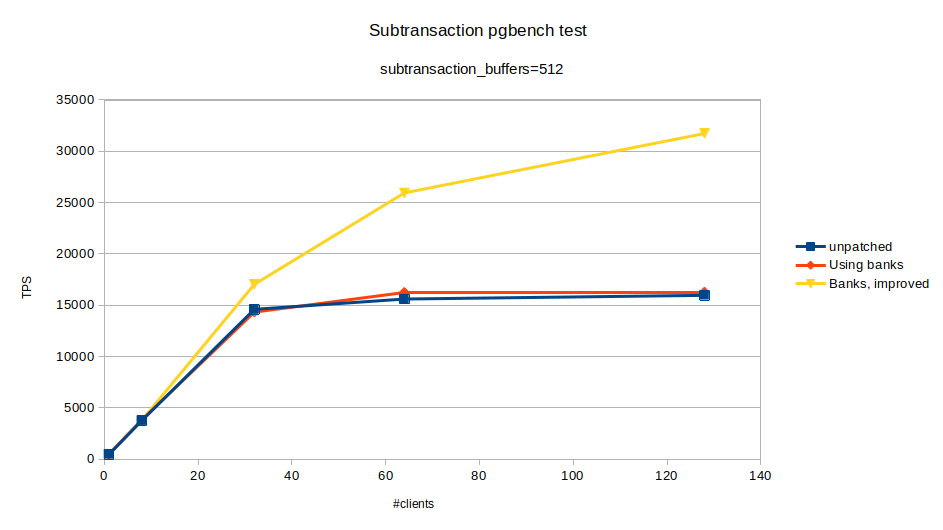
\includegraphics[width=0.9\textwidth]{subtrans-tps.png}
\end{frame}

\begin{frame}
  \frametitle{Multixact TPS improvement}
  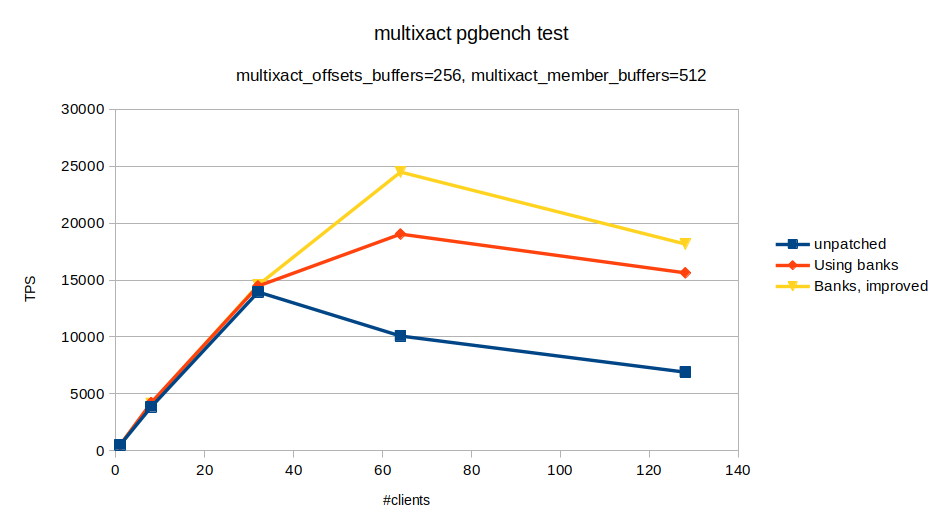
\includegraphics[width=0.9\textwidth]{multixact-tps.png}
\end{frame}


\begin{frame}
  \frametitle{Performance Fixes in Postgres 17}
  \begin{itemize}
    \item {\linksize \href{https://git.postgresql.org/cgit/postgresql.git/commit/?id=d172b717c6f436738cc8383a4e9f611ae227fd93}
      {Commit d172b717c6f4: \faExternalLink \\
      Use atomic access for SlruShared->latest\_page\_number \\
      Dilip Kumar (via Álvaro Herrera) \\
      Tue Feb 6 2024, Postgres 17}}
      \vspace{0.2cm}
    \item {\linksize \href{https://git.postgresql.org/cgit/postgresql.git/commit/?id=53c2a97a92665be6bd7d70bd62ae6158fe4db96e}
      {Commit 53c2a97a9266: \faExternalLink \\
      Improve performance of subsystems on top of SLRU \\
      Andrey Borodin and Dilip Kumar (via Álvaro Herrera) \\
      Wed Feb 28 2024, Postgres 17}}
  \end{itemize}
\end{frame}

\begin{frame}[fragile]
  \frametitle{The New GUCs}
  \begin{itemize}
    \item A few must be set to nonzero values, defaults similar as before
    \item Up to 1024~MB in multiples of 16 (the bank size)
  \end{itemize}
  \begin{lstlisting}[frame=trBL,frameround=fttt]
# SLRU buffers (change requires restart)
multixact_offset_buffers = 16
multixact_member_buffers = 32
notify_buffers = 16
serializable_buffers = 32
  \end{lstlisting}  
\end{frame}

\begin{frame}[fragile]
  \frametitle{The New GUCs: autoscaling}
  \begin{itemize}
    \item A few are automatically derived from \texttt{shared\_buffers}
  \end{itemize}
  \begin{lstlisting}[frame=trBL,frameround=fttt]
# SLRU buffers (change requires restart)
commit_timestamp_buffers = 0
subtransaction_buffers = 0
transaction_buffers = 0
  \end{lstlisting}  
  \begin{itemize}
    \item 2 MB for each 1024 MB of shared\_buffers
    \item Up to a maximum of 8 MB
    \item Can still be set manually
  \end{itemize}
\end{frame}

\begin{frame}
  \frametitle{Action Items for Postgres DBAs}

  \begin{itemize}
    \item Add \texttt{pg\_stat\_slru} to monitoring
    \item Upgrade to Postgres 17
    \item Track whether any of the SLRUs need to be reconfigured
  \end{itemize}
\end{frame}

\begin{frame}[fragile]
  \frametitle{Suggested Monitoring Query}

  \begin{lstlisting}[frame=trBL,frameround=fttt]
  SELECT name, blks_zeroed, blks_read,
       blks_hit+blks_read AS blks_accessed,
       CASE WHEN blks_hit+blks_read = 0 THEN 'NaN'
       ELSE (blks_hit::numeric / (blks_hit+blks_read))
            ::numeric(4,2) END AS hit_ratio
    FROM pg_stat_slru;
  \end{lstlisting}
\end{frame}

\begin{frame}
  \frametitle{Another Talk on this Topic}
\noindent  \href{https://www.pgevents.ca/events/pgconfdev2024/schedule/session/53-problem-in-postgresql-slru-and-how-we-are-optimizing-it/}
  {``SLRU Performance Issues: How we have optimized it'',\\
  Dilip Kumar, PGConf.dev 2024 \faExternalLink}
  \center 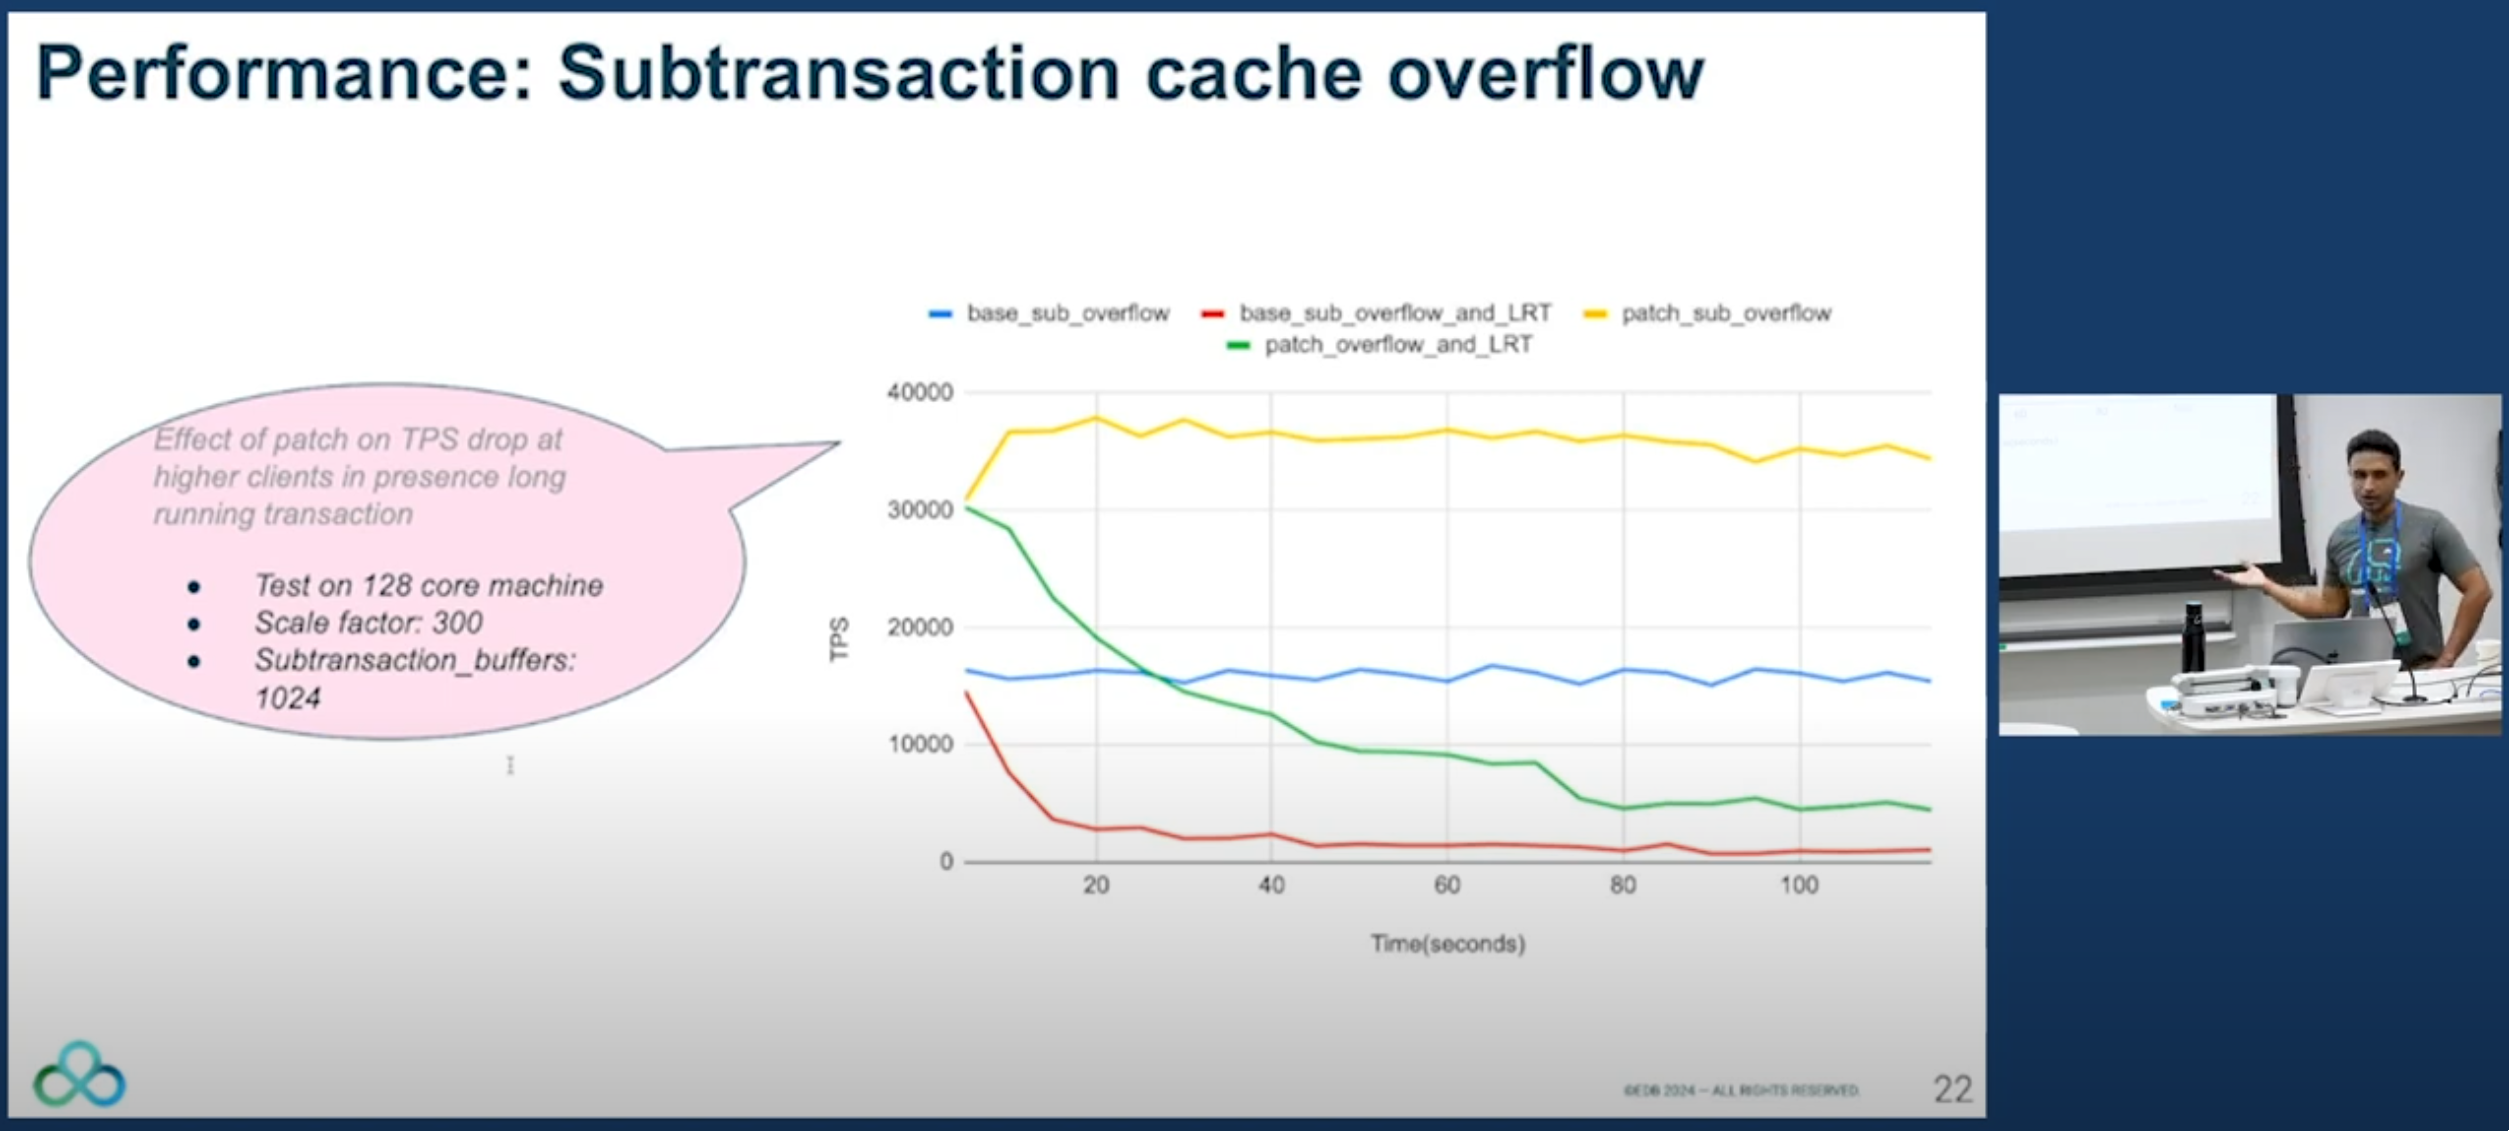
\includegraphics[width=0.8\textwidth]{dilip.png}
\end{frame}

\begin{frame}
  \frametitle{Future Work}
  \begin{itemize}
    \item Use per-bank LRU counters
      \begin{itemize}
	\item avoids latency of atomic ops
      \end{itemize}
    \item Improve LRU algorithm
      \begin{itemize}
	\item Ants Aasma has better code
	\item I'm especially hoping it'll avoid my stupid use of integer division
      \end{itemize}
  \end{itemize}
\end{frame}
